\documentclass[unicode,11pt,a4paper,oneside,numbers=endperiod,openany]{scrartcl}

\usepackage{xcolor}
\usepackage{listings}
\usepackage{amsmath}

% Define custom verbatim environment with gray background
\lstnewenvironment{grayverbatim}{%
  \lstset{backgroundcolor=\color{gray!10}, % Adjust the shade of gray as desired
          frame=single,
          framerule=0pt,
          basicstyle=\ttfamily,
          breaklines=true,
          columns=fullflexible}
}{}

\lstnewenvironment{cppverbatim}{%
  \lstset{language=C++, % Set the language to C++
          backgroundcolor=\color{gray!10}, % Adjust the shade of gray as desired
          frame=single,
          framerule=0pt,
          basicstyle=\ttfamily,
          keywordstyle=\color{blue}, % Set the color for keywords
          commentstyle=\color{green!50!black}, % Set the color for comments
          stringstyle=\color{red}, % Set the color for strings
          breaklines=true,
          showstringspaces=false, % Don't show spaces within strings
          columns=fullflexible}
}{}

\usepackage{ifthen}
\usepackage[utf8]{inputenc}
\usepackage{graphics}
\usepackage{graphicx}
\usepackage{hyperref}

\pagestyle{plain}
\voffset -5mm
\oddsidemargin  0mm
\evensidemargin -11mm
\marginparwidth 2cm
\marginparsep 0pt
\topmargin 0mm
\headheight 0pt
\headsep 0pt
\topskip 0pt        
\textheight 255mm
\textwidth 165mm

\newcommand{\duedate} {}
\newcommand{\setduedate}[1]{%
\renewcommand\duedate {Due date:~ #1}}
\newcommand\isassignment {false}
\newcommand{\setassignment}{\renewcommand\isassignment {true}}
\newcommand{\ifassignment}[1]{\ifthenelse{\boolean{\isassignment}}{#1}{}}
\newcommand{\ifnotassignment}[1]{\ifthenelse{\boolean{\isassignment}}{}{#1}}

\newcommand{\assignmentpolicy}{
\begin{table}[h]
\begin{center}
\scalebox{0.8} {%
\begin{tabular}{|p{0.02cm}p{16cm}|}
\hline
&\\
\multicolumn{2}{|c|}{\Large\textbf{HPC Lab for CSE 2024 ---  Submission Instructions}}\\
\multicolumn{2}{|c|}{\large\textbf{(Please, notice that following instructions are mandatory: }}\\
\multicolumn{2}{|c|}{\large\textbf{submissions that don't comply with, won't be considered)}}\\
&\\
\textbullet & Assignments must be submitted to \href{https://moodle-app2.let.ethz.ch/course/view.php?id=22516}{Moodle} (i.e. in electronic format).\\
\textbullet & Provide both executable package and sources (e.g. C/C++ files, Matlab). 
If you are using libraries, please add them in the file. Sources must be organized in directories called:\\
\multicolumn{2}{|c|}{\textit{Project\_number\_lastname\_firstname}}\\
& and  the  file must be called:\\
\multicolumn{2}{|c|}{\textit{project\_number\_lastname\_firstname.zip}}\\
\multicolumn{2}{|c|}{\textit{project\_number\_lastname\_firstname.pdf}}\\
\textbullet &  The TAs will grade your project by reviewing your project write-up, and looking at the implementation 
                 you attempted, and benchmarking your code's performance.\\

\textbullet & You are allowed to discuss all questions with anyone you like; however: (i) your submission must list anyone you discussed problems with and (ii) you must write up your submission independently.\\
\hline
\end{tabular}
}
\end{center}
\end{table}
}
\newcommand{\punkte}[1]{\hspace{1ex}\emph{\mdseries\hfill(#1~\ifcase#1{Points}\or{Points}\else{Points}\fi)}}


\newcommand\serieheader[6]{
\thispagestyle{empty}%
\begin{flushleft}

\includegraphics[width=0.4\textwidth]{ETHlogo_13}
\end{flushleft}
  \noindent%
  {\large\ignorespaces{\textbf{#1}}\hspace{\fill}\ignorespaces{ \textbf{#2}}}\\ \\%
  {\large\ignorespaces #3 \hspace{\fill}\ignorespaces #4}\\
  \noindent%
  \bigskip
  \hrule\par\bigskip\noindent%
  \bigskip {\ignorespaces {\Large{\textbf{#5}}}
  \hspace{\fill}\ignorespaces \large \ifthenelse{\boolean{\isassignment}}{\duedate}{#6}}
  \hrule\par\bigskip\noindent%  \linebreak
 }

\makeatletter
\def\enumerateMod{\ifnum \@enumdepth >3 \@toodeep\else
      \advance\@enumdepth \@ne
      \edef\@enumctr{enum\romannumeral\the\@enumdepth}\list
      {\csname label\@enumctr\endcsname}{\usecounter
        {\@enumctr}%%%? the following differs from "enumerate"
	\topsep0pt%
	\partopsep0pt%
	\itemsep0pt%
	\def\makelabel##1{\hss\llap{##1}}}\fi}
\let\endenumerateMod =\endlist
\makeatother




\usepackage{textcomp}






\begin{document}


\setassignment
\setduedate{Monday 15 April 2024, 23:59 (midnight)}

\serieheader{High-Performance Computing Lab for CSE}{2024}
            {Student: CARLA JUDITH LOPEZ ZURITA}
            {Discussed with: FULL NAME}{Solution for Project 3}{}
\newline

\assignmentpolicy

In this report, we are solving Fisher's equation using the finite difference
method. The equation is given by:
\begin{align}
    \frac{\partial s}{\partial t} = D \nabla^2 u + R s (1 - s)
\end{align}
where $s$ is the concentration of a species, $D$ is the diffusion coefficient,
and $R$ is the reaction rate. The equation is solved on a 2D grid with
Dirichlet boundary conditions,
\begin{align}
    s(x, y, t) = 0.1 \quad \text{for} \quad x = 0, x = 1, y = 0, y = 1
\end{align}
and initial conditions is a circle of radius $1/8$ at the lower left quadrant the domain.
\section{Task: Implementing the linear algebra functions and the stencil
         operators [40 Points]}

The first part of the project consists in implementing the linear algebra functions and
the stencil operators. The linear algebra functions are implemented in the
\texttt{linalg.cpp} file. I implemented all the functions using
simple loops.
%  I tried using iterators but since the Fields class is a custom
% class, I decided to put that idea on hold until I have a better understanding of
% the code. 
Similarly, the stencil operators were implemented in the
\texttt{operators.cpp} file. Writing the interior grid points was very simple since
we already had the implementations for the boundary conditions.

Afterwards, I ran the code following the indications on the project description
and I got the following results in the terminal
\begin{grayverbatim}
================================================================================
                      Welcome to mini-stencil!
version   :: C++ Serial
mesh      :: 128 * 128 dx = 0.00787402
time      :: 100 time steps from 0 .. 0.005
iteration :: CG 300, Newton 50, tolerance 1e-06
================================================================================
--------------------------------------------------------------------------------
simulation took 0.203392 seconds
1513 conjugate gradient iterations, at rate of 7438.82 iters/second
300 newton iterations
--------------------------------------------------------------------------------
### 1, 128, 100, 1513, 300, 0.203392 ###
Goodbye!
\end{grayverbatim}
Which are the expected results, even if a bit slower than the results included
in the original document, but this is just one run and could be attributed to
the randomness of run-time of the processes. Additionally, I got the following content for
the \texttt{output.bin} file,
\begin{grayverbatim}
TIME: 0.005
DATA_FILE: output.bin
DATA_SIZE: 128 128 1
DATA_FORMAT: DOUBLE
VARIABLE: phi
DATA_ENDIAN: LITTLE
CENTERING: nodal
BRICK_ORIGIN: 0. 0. 0.
BRICK_SIZE: 1 1  1.0
\end{grayverbatim}
which produced Fig. \ref{im:final_time}.
\begin{figure}[h]
    \centering
    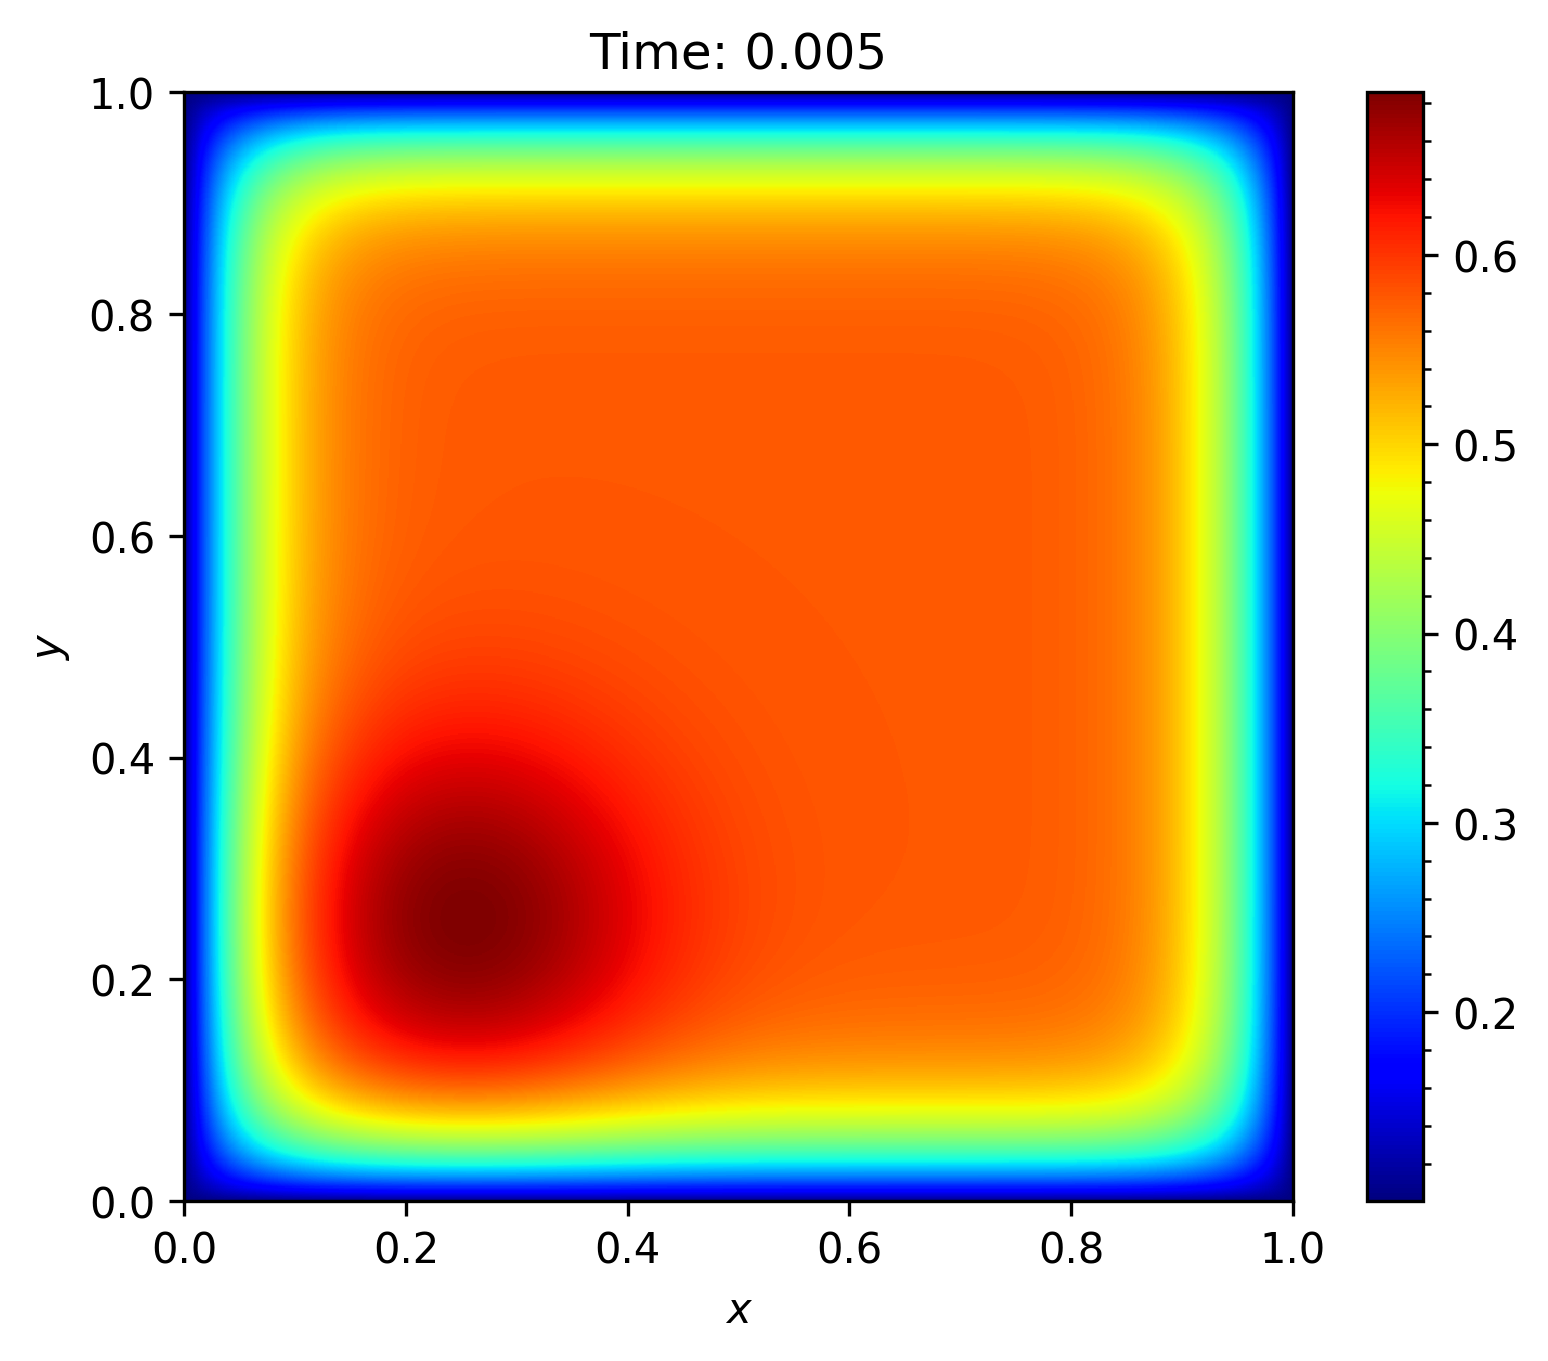
\includegraphics[width=0.5\textwidth]{../mini_app/output.png}
    \caption{The population concentration at time t = 0.005.}
    \label{im:final_time}
\end{figure}

\section{Task:  Adding OpenMP to the nonlinear PDE mini-app [60 Points]}
This section is dedicated to parallelizing the code using OpenMP. 

\subsection*{Welcome message and serial compilation}
We want to have different welcome messages for the serial and parallel versions.
This was done using the macro \texttt{\_OPENMP} which is defined when OpenMP is
enabled. The code is shown below.
\begin{cppverbatim}
#ifdef _OPENMP
#include "omp.h" // This line won't add the library if you don't compile with -fopenmp option.
#endif

...

#ifdef _OPENMP
    std::cout << "version   :: C++ OpenMP" << std::endl;
#pragma omp parallel
    {
        threads = omp_get_num_threads();
    }
    std::cout << "threads   :: " << threads << std::endl;
#else
    std::cout << "version   :: C++ Serial" << std::endl;
#endif
\end{cppverbatim}    
This seems to work as expected. The code is compiled with the \texttt{-fopenmp}
flag to enable OpenMP.

\subsection*{Linear algebra kernel}
Afterwards, the first step to parallelize the code was to work on the linear algebra functions. I used simple \texttt{omp
parallel for} directive to parallelize the loops.

\subsection*{The diffusion stencil}
Then, I parallelized the
stencil operators. I used the same directive as before. 

\subsection*{Bitwise identical results}
I converted the bin files to hex files to be able to see clearly if the parallel
implementation was producing bitwise identical results. The reults was that they
were not identical.

TODO: Discuss

\subsection*{Strong scaling}
Next, we want to analyze the performance of the code. We will analyze the strong
and weak scaling of the code. I repeated the runs 100 times for the serial and
50 for the parallel
versions to get better timing results.
It was a bit challenging to be able to determine the run time for certain using
only one run, since there seemed to be a lot of variability in the run times.
The codes to compile and run the experiments are included in the bash scripts
accompanying this report. We can see the distribution of the run times in Fig. \ref{im:times}.
\begin{figure}
    \centering
    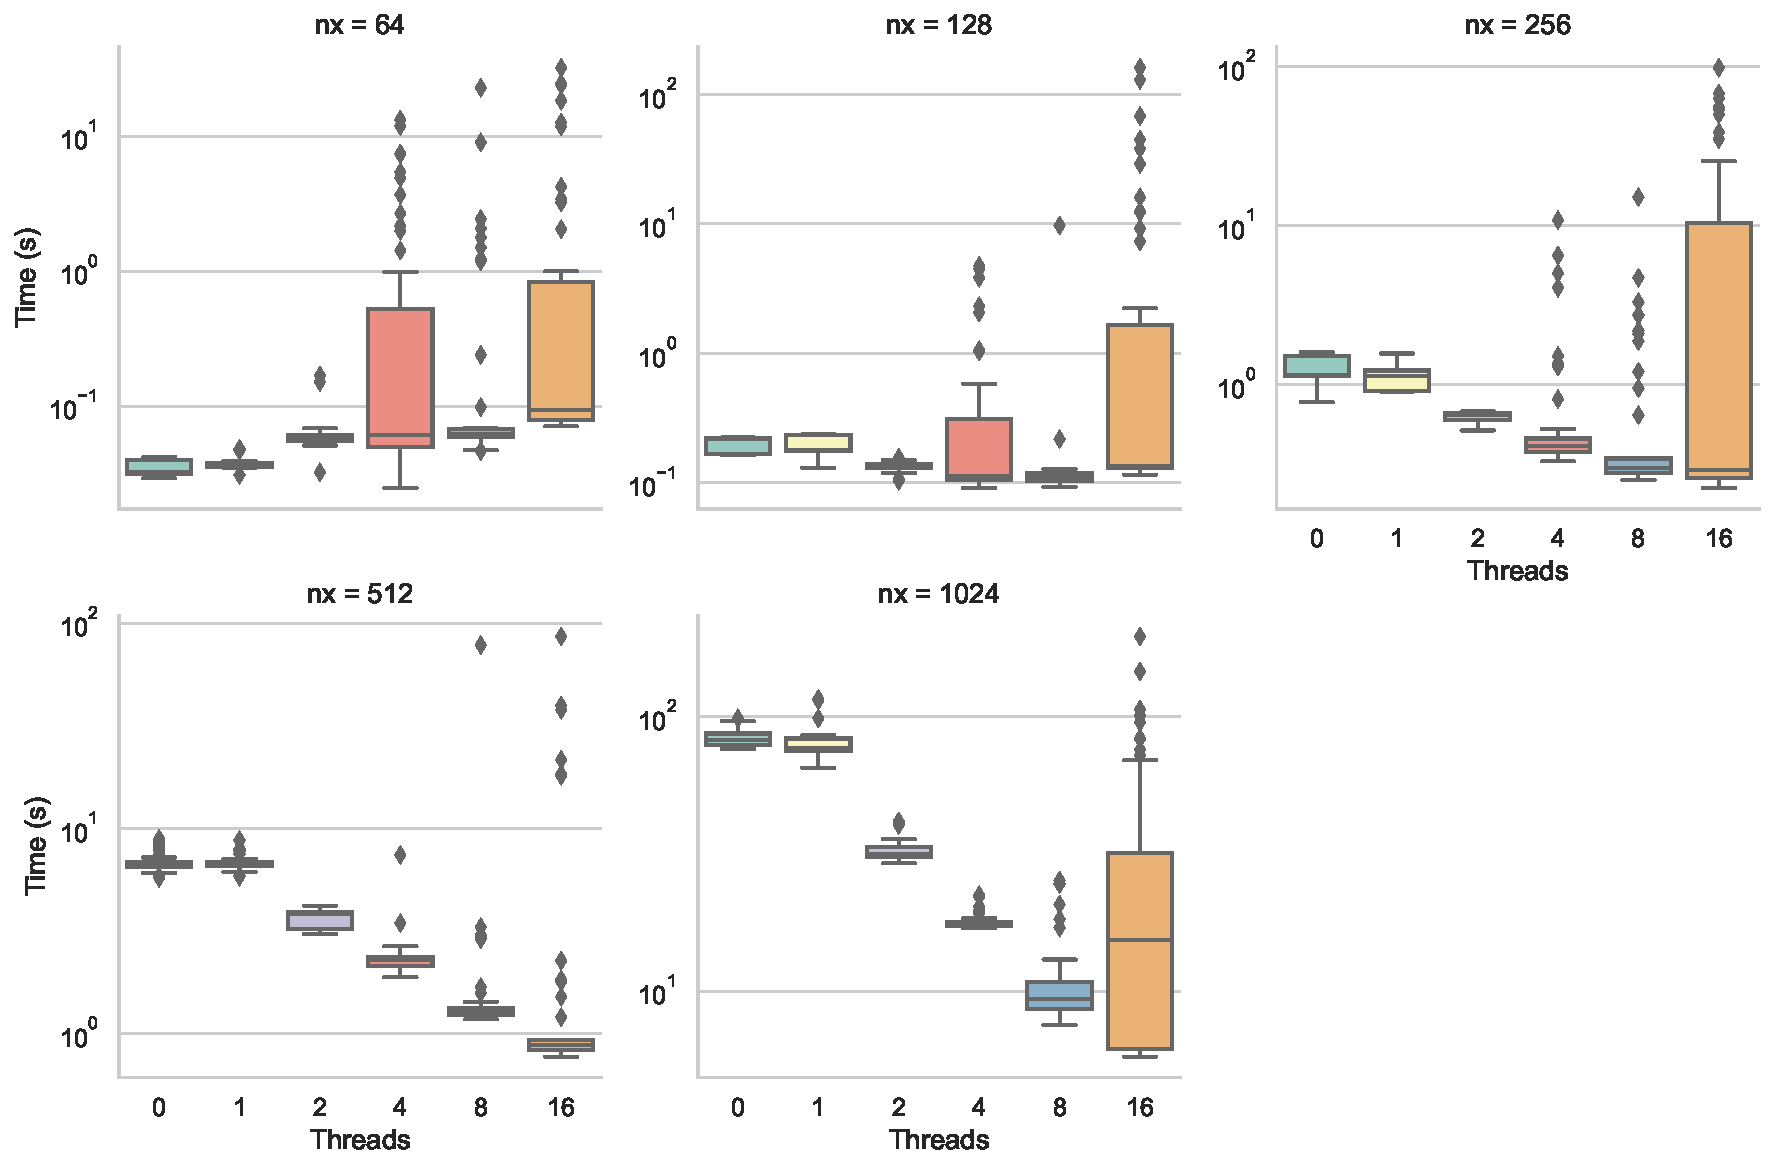
\includegraphics[width=\textwidth]{../mini_app/data_var.pdf}
    \caption{Time taken for the serial and parallel versions of the code; zero threads indicates serial version.}
    \label{im:times}
\end{figure}
Since the run times are so variable, I decided to use the median of the run
times
to determine the run time for the strong and weak scaling experiments. The
results
are shown in Figs. \ref{im:strong_scaling}
\begin{figure}
    \centering
    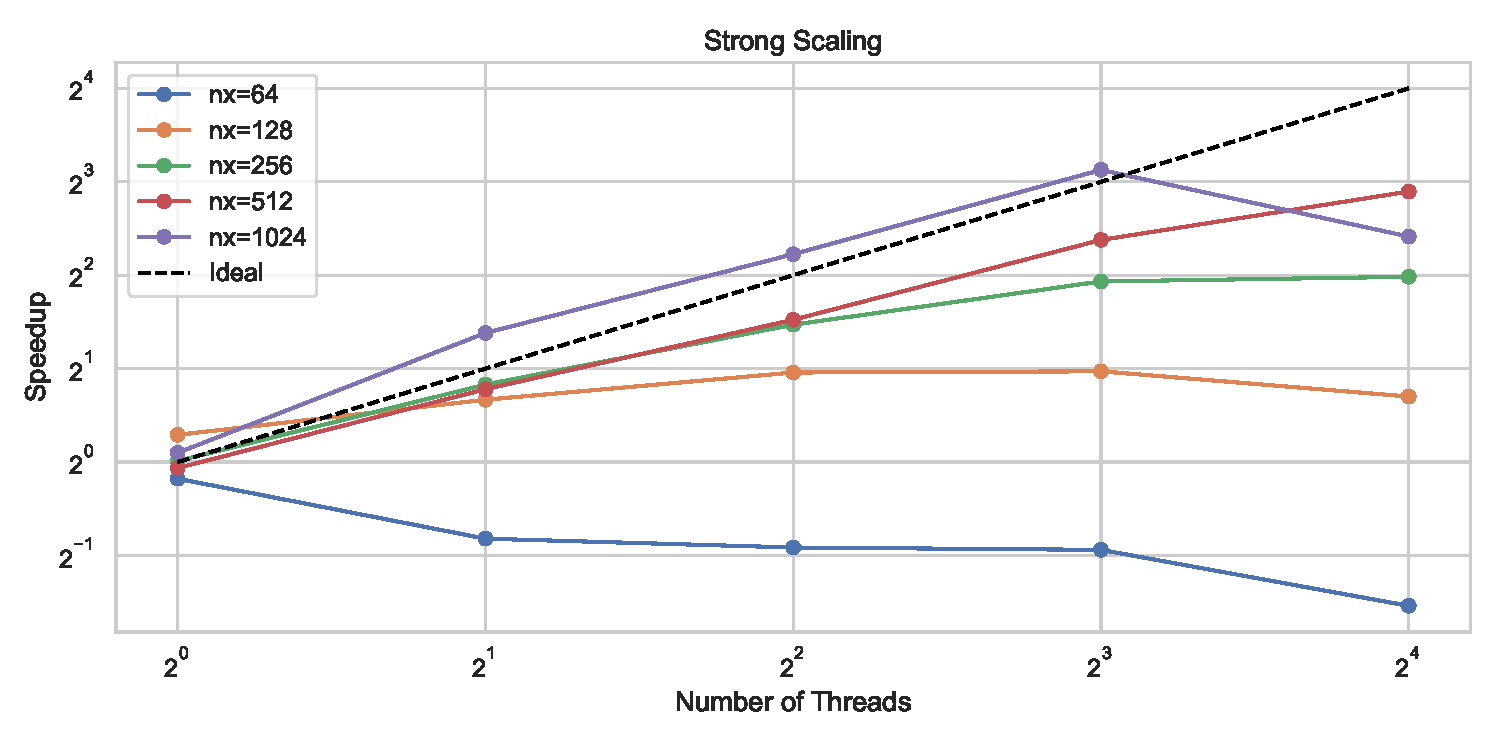
\includegraphics[width=\textwidth]{../mini_app/strong_scaling_plot.pdf}
    \caption{Strong scaling of the code.}
    \label{im:strong_scaling}
\end{figure}

\subsection*{Weak scaling}
For the weak scaling, I ran the code for the parallel verison 100 times for each
combination of threads and grid size. The results are shown in Fig.
\ref{im:weak_scaling}. I followed the same procedure as for the strong scaling
to determine the run time.

\begin{figure}
    \centering
    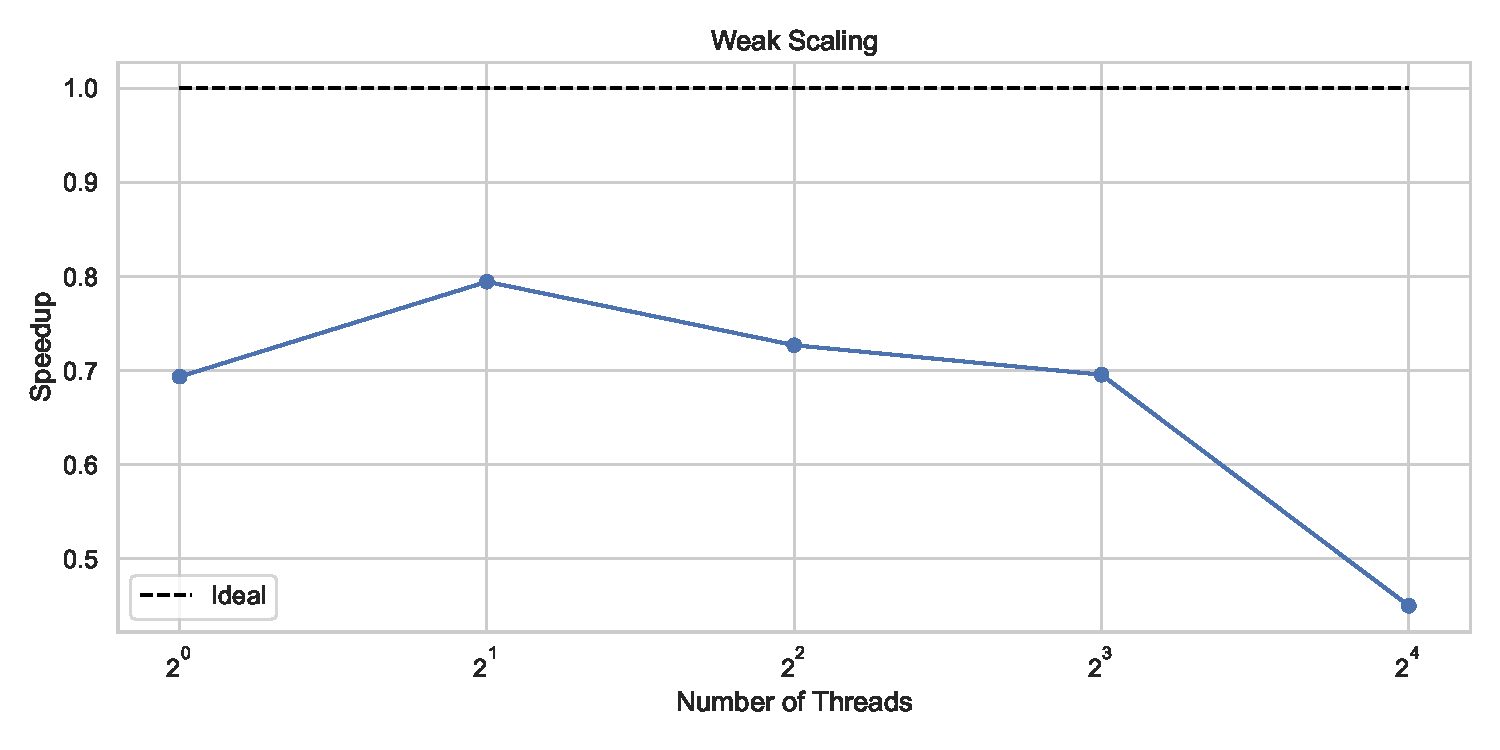
\includegraphics[width=\textwidth]{../mini_app/weak_scaling_plot.pdf}
    \caption{Weak scaling of the code.}
    \label{im:weak_scaling}
\end{figure}


\end{document}
